\section{Dokumentation der jExam Testinfrastruktur}

\subsection{Über die Testinfrastruktur}

Das Ziel dieses Projekts ist die Entwicklung einer
vollautomatischen automatisierte Testinfrastruktur
zum Testen der jExam-Plattform zu schaffen. In ihrem
derzeitigen Zustand umfasst die Test Testinfrastruktur
Leistungstests, Sicherheitstests Sicherheitstests
und funktionale UI-Tests. Der Projektcode ist eine
Grundlage für die Entwicklung von Tests für die der
jExam-Plattform und muss in den nächsten Monaten und
Jahren weiterentwickelt Monaten und Jahren
weiterentwickelt und gepflegt werden.

\subsection{Verwendete Technologien}

Zum Erstellen der Testinfrastruktur:

\textbf{Docker} (Stellen Sie sicher, dass Sie
Docker auf Ihrem Gerät installiert haben)


Für UI-Tests:
\begin{enumerate}
    \item \textbf{Selenium}
    \item \textbf{TestNG}
    \item \textbf{AssertJ - fluent assertions java library}
    \item \textbf{Extent Reports}

\end{enumerate}

Für Leistungstests:

\textbf{JMeter}

Für Sicherheitstests:

\textbf{ZAP Proxy}

Um die Skripte ändern zu können oder Fehler zu
verstehen, die in Zukunft auftreten könnten, ist
es für den Tester unerlässlich, Grundkenntnisse
über die oben genannten Technologien zu haben.

\subsection{Einrichtung des Projekts}

Klonen Sie das Repository mit :
\begin{lstlisting}[caption={Clone repository},label={lst:clone repo}]
git clone ssh://ipra38.inf.tu-dresden.de/jexam/jexam-webtest.git
\end{lstlisting}

Die allgemeine Struktur der Docker-Infrastruktur
sieht folgendermaßen aus:

\begin{figure}[H]
    \centering
    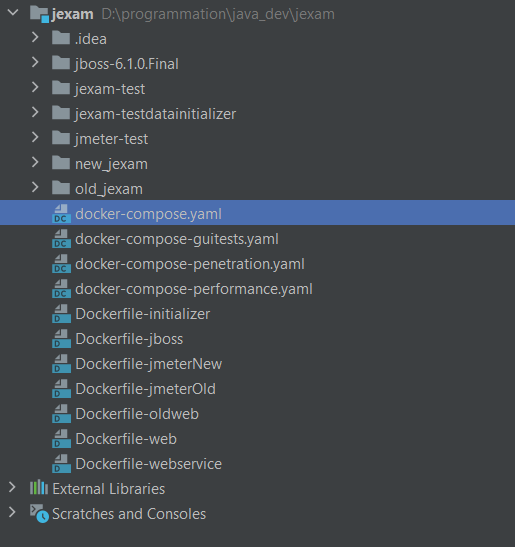
\includegraphics[scale=1]{images/docker-files}
    \caption{Globale Dateistruktur der jExam-Testinfrastruktur} \label{fig:global}
\end{figure}

\begin{enumerate}

    \item \textbf{jboss-6.1.0.Final} : Dieser Ordner
    enthält den Quellcode zum Starten des jboss-Servers, der von der jExam-Infrastruktur verwendet wird.

    \item \textbf{jexam-test}: Dieser Ordner ist das
    Selenium-Projekt, das die UI-Tests enthält.

    \item \textbf{jexam-testdatainitializer}: Dieser
    Ordner enthält das Java-Skript zum Einspeisen der
    Daten in den jboss-Server.

    \item \textbf{jmeter-test}: Dieser Ordner enthält
    das jmeter-Skript, das für Leistungstests nützlich
    ist.

    \item \textbf{new\_jexam und old\_jexam}: Diese
    Ordner enthalten den Quellcode der neuen bzw.
    alten Version der jExam-Webanwendung.

\end{enumerate}

\subsection{jExam-Anwendungen starten}

Bevor ein Skript ausgeführt werden kann, muss
zunächst Docker gestartet werden. Wenn dies
geschehen ist, muss der Tester ein Docker-Netzwerk
mit dem Befehl erstellen:

\begin{lstlisting}[caption={Docker Network Einrichtung}]
docker network create jexam_network
\end{lstlisting}

Sobald das Netzwerk erstellt ist, soll der Tester
den folgenden Befehl ausführen:

\begin{lstlisting}[caption={Befehl zum Starten der jExam-Plattformen}]
docker-compose up

/* oder wenn  Änderungen in einem der folgenden Ordner vorgenommen wurden (jboss-6.1.0.Final, old_jexam, new_jexam, jexam-testdatainitializer): */

docker-compose up --build
\end{lstlisting}

Dies ermöglicht die Ausführung von jExam 2009 und jExam
New, die über die folgenden Links aufgerufen werden können:

\begin{itemize}
    \item[] \textbf{jExam 2009} : http://localhost:8085/web/
    \item[] \textbf{jExam New} : http://localhost:8080/
\end{itemize}

Nach der Ausführung des Skripts erzeugt der
Initialisierer eine csv-Datei, die unter
jexam-test/initializer-csv/testData.csv
zugänglich ist und alle Testdaten enthält,
die in den JBoss-Server eingespeist wurden.


\subsection{Durchführung von Performancetests}

Die Durchführung der Performancetests erfordert die
Ausführung des folgenden Befehls:

\begin{lstlisting}[caption={Befehl zur Durchführung der Performancetests}]
docker-compose -f  docker-compose-performance.yaml up

/* oder wenn  Änderungen in jmeter-test Ordner vorgenommen wurden: */

docker-compose -f  docker-compose-performance.yaml up --build
\end{lstlisting}

Im Ordner jmeter-test/tests befinden sich die
Dateien jExam\_new.jmx und jExam\_old.jmx, die
jeweils die JMeter-Tests für die Plattformen
jExam New und jExam 2009 enthalten. Nach der
Ausführung der Tests wird ein Bericht erstellt, der
vom Tester in:
\begin{itemize}
    \item[] \textbf{jExam 2009} : jexam-test/jmeter-newjexam-test-output
    \item[] \textbf{jExam New} : jexam-test/jmeter-oldjexam-test-output
\end{itemize}

\begin{figure}[H]
    \centering
    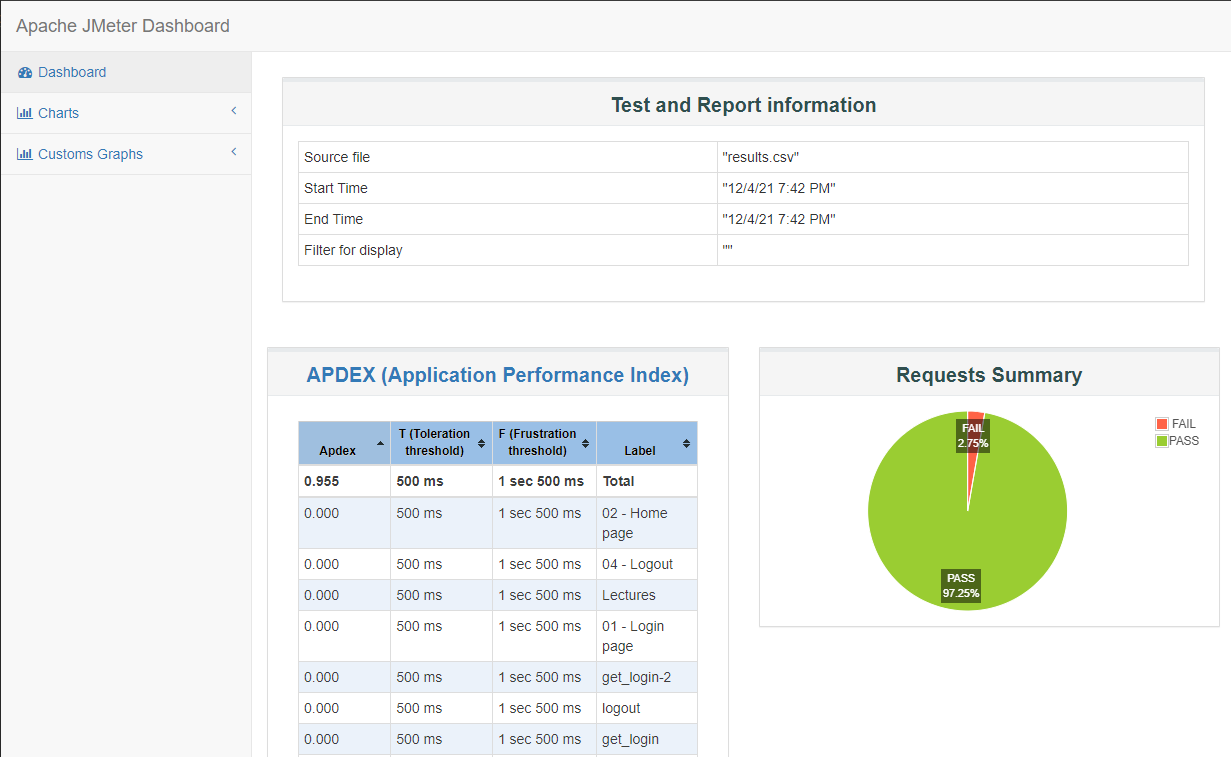
\includegraphics[scale=0.4]{images/jmeter-report}
    \caption{Beispiel für einen JMeter-Bericht} \label{fig:jmeter-report}
\end{figure}

\subsection{Durchführung von Sicherheitstests}

Die Durchführung der Sicherheitstests erfordert die
Ausführung des folgenden Befehls:

\begin{lstlisting}[caption={Befehl zur Durchführung der Sicherheitstests}]
docker-compose -f  docker-compose-penetration.yaml up

/* oder wenn  Änderungen in docker-compose-penetration.yaml Datei vorgenommen wurden: */

docker-compose -f  docker-compose-penetration.yaml up --build
\end{lstlisting}

Es gibt zwei mögliche ausführbare Skripte für
Sicherheitstests: ZAP-Baseline und ZAP-Fullscann.
Der Tester muss im Voraus auswählen, welches Skript
er für welche Anwendung ausführen möchte. Zu diesem
Zweck muss er die Datei
\textbf{docker-compose-penetration.yaml} ändern:

\begin{lstlisting}[caption={docker-compose-penetration.yaml}]

command: [ "./wait-for-it.sh", "web:8080", "bash" ,"-c", "zap-baseline.py -t http://web:8080 -r owaspReport.html" ]
# web:8080 for jExam New and oldweb:8080 for jExam 2009
# "zap-baseine.py -t" for ZAP-Baseline scan or
# "zap-full-scan.py -d -j -m 1 -t" for ZAP-Fullscan
\end{lstlisting}

Der von der Testausführung erstellte Bericht ist
im Ordner jexam-test/owasp-test-output verfügbar.

\begin{figure}[H]
    \centering
    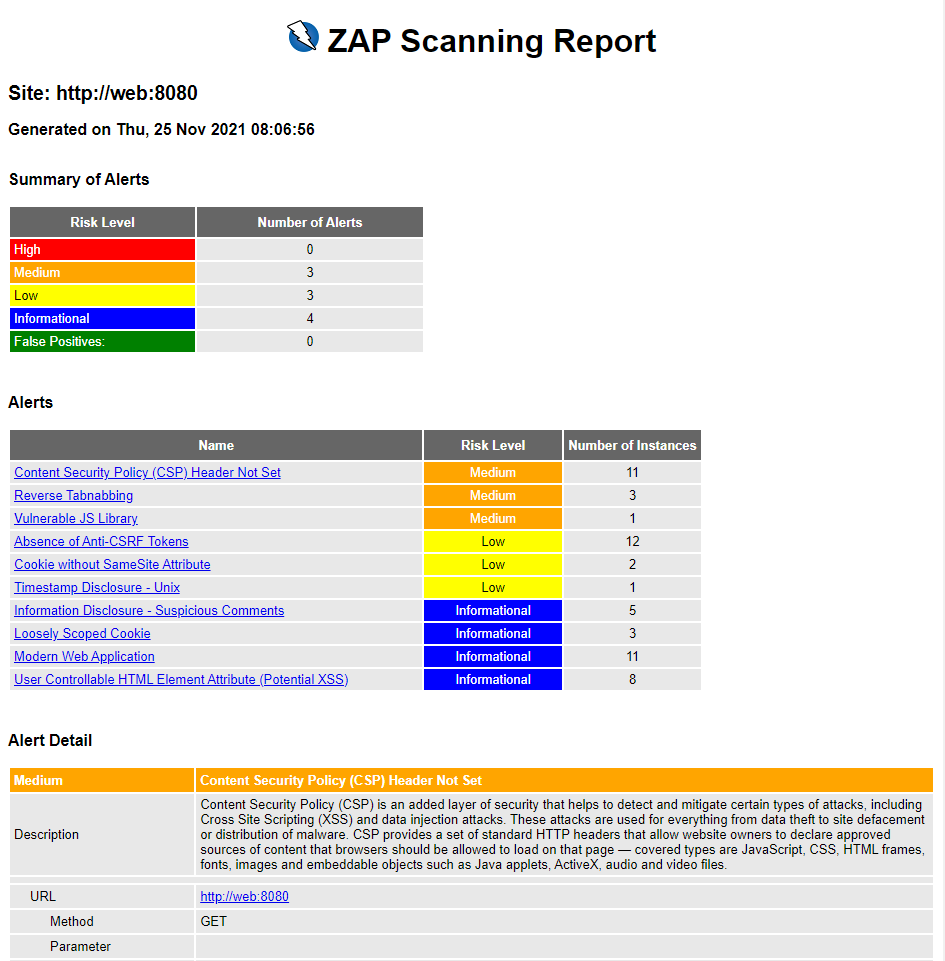
\includegraphics[scale=0.5]{images/zap-report}
    \caption{Beispiel für einen ZAP Proxy-Bericht} \label{fig:zap-report}
\end{figure}

\subsection{Durchführung von Seleniumtests}

Vor der Ausführung der Tests muss der Tester
unbedingt die vom jexam-testdatainitializer
bereitgestellten Testdaten einrichten. Der Tester
muss die Daten aus der
Datei jexam-test/initializer-csv/testData.csv in die
Java-Klasse
jexam-test/src/test/java/jexam/web/test/entities/TestUser.java
kopieren.

\begin{figure}[H]
    \centering
    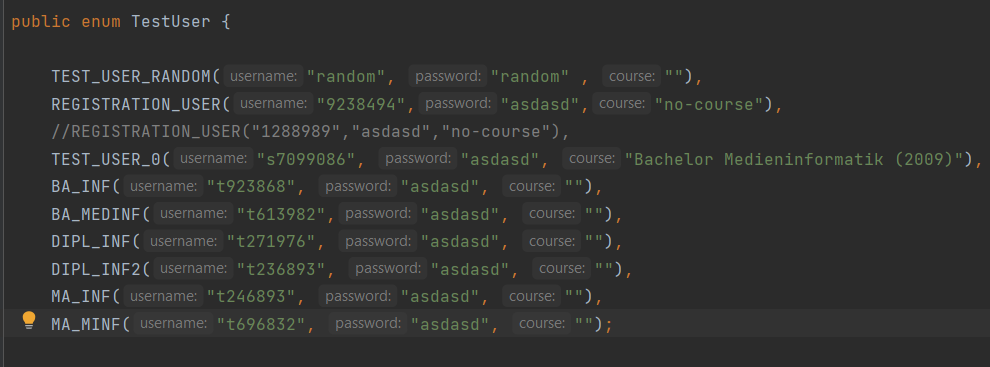
\includegraphics[scale=0.5]{images/test-data}
    \caption{TestUser Java Class}\label{fig:testUser}
\end{figure}


\subsubsection{Ausführungsmodus}

Es gibt zwei Ausführungsmodi für UI-Tests, nämlich
den \textbf{lokalen} Modus und den \textbf{Remote}
Modus.

Der \textbf{lokale} Modus ist der Modus, den der
Tester bei der Entwicklung der Tests verwendet.
Der Hauptvorteil dieses Modus ist, dass er
eine schnelle Testausführung ermöglicht und
keinen Remote-Webdriver erfordert.

Um die Tests im lokalen Modus auszuführen, muss der
Tester in die Datei
jexam/jexam-test/src/test/resources/config/config.properties
gehen und dort einige Anpassungen vornehmen:

\begin{lstlisting}[caption={config.properties}]
#Browser (chrome or firefox)
browser=chrome

#run mode (local) --> Jexam version (LOCAL_WEB for jExam New, LOCAL_OLDWEB for jExam 2009)
#run mode (remote) ---> Jexam version (WEB jExam New, OLDWEB for jExam 2009)
runmode=local

# Jexam version (WEB, OLDWEB, LOCAL_WEB, LOCAL_OLDWEB)
jexam_version = LOCAL_WEB

seleniumgridurl=http://selenium-hub:4444/wd/hub

#headless or not
headless=false

overridereports = yes

\end{lstlisting}

Nach der Konfiguration muss der Tester den folgenden
Befehl im jexam-test-Ordner ausführen:

\begin{lstlisting}[caption={Maven Test Command}]
mvn clean test
\end{lstlisting}

Der \textbf{remote} Modus wird hauptsächlich für die
Ausführung von Tests in Docker-Containern verwendet.
Um ihn zu verwenden, muss der Tester auch
Anpassungen in der Datei
jexam/jexam-test/src/test/resources/config/config.properties
vornehmen. Zum Beispiel:

\begin{lstlisting}[caption={config.properties}]
runmode=remote
jexam_version=WEB
\end{lstlisting}

Der Tester sollte den folgenden Befehl in der
Stammdatei der Testinfrastruktur verwenden, um sie
im Remote-Modus in Docker-Containern auszuführen und am
Ende der Testausführung wird ein Extent-Bericht
erstellt, der im Ordner jexam-test/extent-test-output
verfügbar ist.

\begin{lstlisting}[caption={docker-compose execution command}]
docker-compose -f  docker-compose-guitests.yaml up --build
\end{lstlisting}

